\section{Results}
\subsection{How many electrodes meet the mean performance tolerance?}
Under the primary curve protocol, full16 achieved mean Macro-F1 \RevPrimaryFull\ and SHAP12 achieved \RevShapMean. The smallest count meeting the 0.02 margin was \KStarMarginPtTwo, with paired change \RevShapDelta\ (95\% CI \RevShapLow\ to \RevShapHigh). Eleven did not meet this criterion: change \DeltaKEleven\ (\DeltaKElevenLCB\ to \DeltaKElevenUCB). The original percentile decision and the exploratory null-centred, Holm-adjusted sensitivity gave the same primary minimum count: \KStarMarginPtOne, \KStarMarginPtTwo\ and \KStarMarginPtThree\ at margins 0.01, 0.02 and 0.03, respectively. The original four penalty curves did not change these count decisions (figure~\ref{fig:ni}; full results in the Supplementary).

Mean preservation did not extend uniformly to individuals. For SHAP12 minus full16, the median change was \RevMedianLoss\ and participant SD was \RevLossSD. \RevImprovedCount\ participant improved, while \RevLossCount\ lost more than 0.02. The worst observed change was \RevWorstLoss\ (participant \RevWorstParticipant), and the best was \RevBestChange. The margin is a mean-level engineering criterion, so these counts do not redefine individual non-inferiority.

\begin{table}[htbp]
\centering\small
\caption{Matched primary protocol: reduced subset minus full16. Each row uses all 43 paired participants, 300 boosting rounds and 200,000 training windows.}\label{tab:primary}
\begin{adjustbox}{max width=\textwidth}
\begin{tabular}{lllll}\toprule
Subset & Mean F1 & $\bar\Delta$ & 95\% CI & NI at 0.02\\\midrule
SHAP12 & 0.528 & -0.0133 & [-0.0160, -0.0106] & yes\\
Geometry12 & 0.522 & -0.0193 & [-0.0254, -0.0132] & no\\
\bottomrule\end{tabular}
\end{adjustbox}
\end{table}

\begin{figure}[htbp]\centering
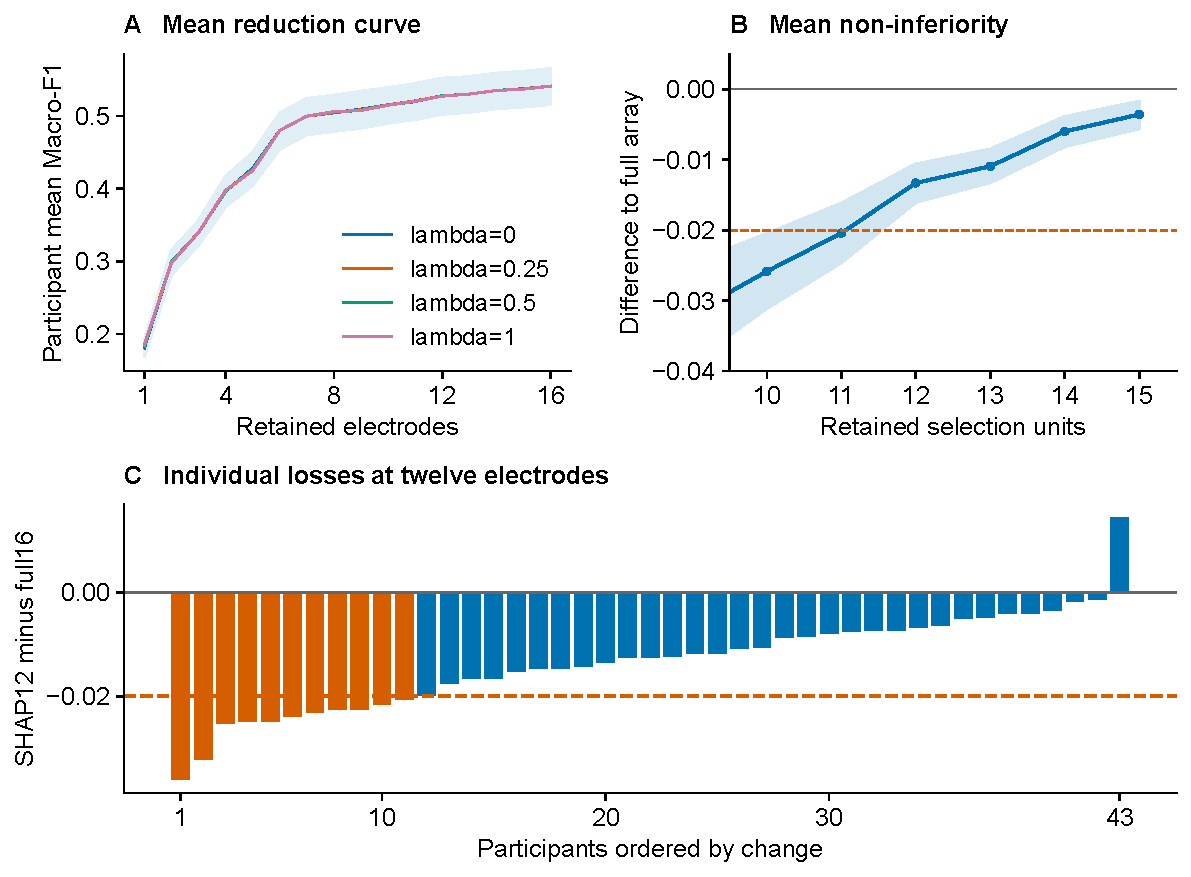
\includegraphics[width=\textwidth]{../figures/vector/fig3_noninferiority.pdf}
\caption{Count reduction and its limits. (A) Participant mean curves for all fixed penalties; shading shows the 95\% participant-bootstrap interval for the unpenalized curve. (B) Mean paired change against the same curve's full16 reference, with 95\% intervals and the 0.02 tolerance. (C) All participant changes at SHAP12, ordered by change; orange identifies observed losses larger than 0.02. The horizontal tolerance in C is a descriptive reference, not an individual inference threshold.}
\label{fig:ni}\end{figure}

\subsection{What does attribution add beyond random and spatial selection?}
In the original lighter-model experiment, attribution-ranked subsets outperformed the participant's mean random-subset baseline at all four tested counts after correction. For the stability-regularized ranking, the mean advantages at counts 4, 6, 8 and 12 were \HTwoKFourDiff, \HTwoKSixDiff, \HTwoKEightDiff\ and \HTwoKTwelveDiff. These absolute scores belong to the lighter comparison model and should not be substituted for the primary non-inferiority curve.

With the primary model and training budget matched, geometric12 scored \RevGeomMean, with change \RevGeomDelta\ (95\% CI \RevGeomLow\ to \RevGeomHigh) from full16. Its lower bound crossed the 0.02 tolerance. The direct SHAP12-minus-geometric12 mean contrast was \RevGeomContrast\ (\RevGeomContrastLow\ to \RevGeomContrastHigh), whose interval included zero. The nominal signed-rank $p=\RevGeomContrastP$ addresses ranks rather than the mean; it does not establish a positive mean advantage. The subsequently completed fixed geometric curve had minimum qualifying counts of \RevGeomKStarCI\ under the percentile rule and \RevGeomKStarNull\ under the null-centred Holm sensitivity at the 0.02 margin; the full curve and decision table are provided in the Supplementary. Different non-inferiority decisions do not establish a difference between methods \citep{gelman2006difference}.

The shared-model comparison is reported separately in table~\ref{tab:matched} and figure~\ref{fig:utility}(C). At counts 6 and 12, SHAP-minus-grouped-permutation mean changes were \RevMatchedSixDiff\ (\RevMatchedSixLow\ to \RevMatchedSixHigh) and \RevMatchedTwelveDiff\ (\RevMatchedTwelveLow\ to \RevMatchedTwelveHigh), with Holm $p\RevMatchedSixP$ and $p\RevMatchedTwelveP$. Mean measured per-outer-fold times were \RevCostTraining\ s for shared inner training, \RevCostShap\ s for SHAP selection and \RevCostPermutation\ s for grouped permutation. These hardware-dependent measurements describe the executed comparison rather than online latency.

At $k=6$, the mean interval supports a positive SHAP advantage; the corrected signed-rank contrast is significant. At $k=12$, the mean advantage remains uncertain because its interval crosses zero; the corrected signed-rank contrast is not statistically detectable.

\begin{table}[htbp]
\centering\small
\caption{Exploratory SHAP minus grouped-electrode permutation. The two methods share the same five inner models and validation observations per outer fold. Holm correction covers the two contrasts.}\label{tab:matched}
\begin{adjustbox}{max width=\textwidth}
\begin{tabular}{llllll}\toprule
$k$ & SHAP & Permutation & $\bar\Delta$ & 95\% CI & $p_{\rm Holm}$\\\midrule
6 & 0.480 & 0.449 & +0.0309 & [+0.0211, +0.0410] & $<0.001$\\
12 & 0.528 & 0.528 & +0.0002 & [-0.0029, +0.0034] & 0.976\\
\bottomrule\end{tabular}
\end{adjustbox}
\end{table}

\begin{figure}[htbp]\centering
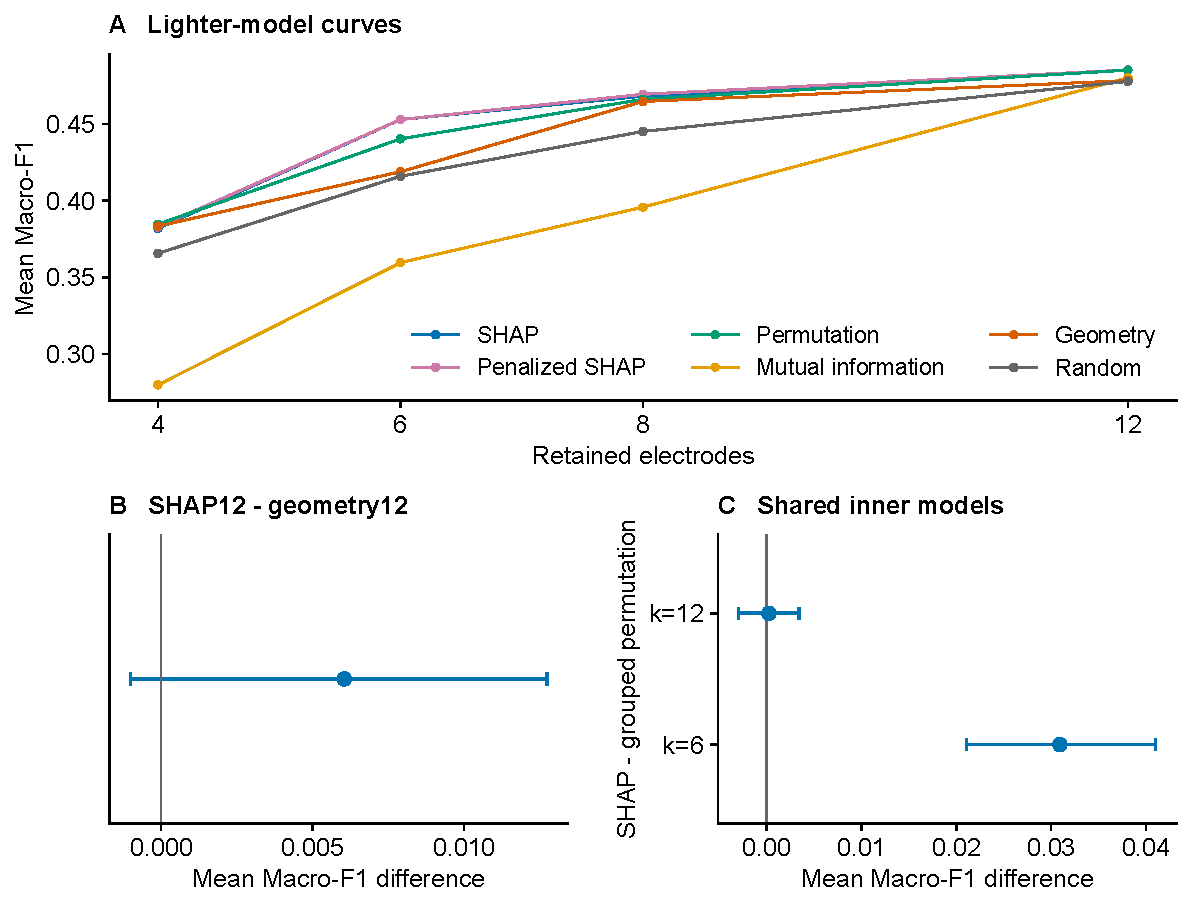
\includegraphics[width=\textwidth]{../figures/vector/fig4_selection_utility.pdf}
\caption{Incremental selection utility under distinct protocols. (A) Historical six-method comparison with a common lighter final classifier (50 boosting rounds, 150,000 training windows); selection-stage resources and validation designs differed, and penalized SHAP uses $\lambda=0.5$. (B) Direct SHAP12-minus-geometric12 mean contrast under the primary protocol (300 boosting rounds, 200,000 windows). (C) SHAP-minus-grouped-permutation contrasts with shared inner models and validation observations and primary-protocol final models. Error bars in B--C are participant mean-change bootstrap intervals. Panels are not a common absolute-score benchmark.}
\label{fig:utility}\end{figure}

\subsection{Which predictive information is lost, and does regularization help?}
Attribution has consistent spatial preferences but does not register sites to individual muscles (figure~\ref{fig:task}(A)). The same top-four set (\TopFourSet) occurred in \TopFourFolds\ outer folds. Outer-fold agreement is descriptive because training cohorts overlap heavily.

The gesture analysis found \RevGestureLossCount\ corrected losses among sixteen active gestures. The largest mean decline was gesture 14, forearm pronation: \RevWorstGestureDelta\ (95\% CI \RevWorstGestureLow\ to \RevWorstGestureHigh). Gestures 2 (thumb adduction), 9 (index finger extension) and 10 (thumb finger extension) also showed corrected declines. These paired gesture-F1 results expose task-specific losses hidden by the global mean; no anatomical cause is inferred from them. Gesture IDs are distinct from electrode indices.

Deletion with retraining produced the expected ordering for the common random-comparison counts: removing highly ranked electrodes gave lower performance than random removal, which gave lower performance than removal of weakly ranked electrodes. At six electrodes retained, Remove-Top minus Remove-Bottom was \FaithTBKSixDiff\ (\FaithTBKSixLCB\ to \FaithTBKSixUCB; Holm $p\FaithTBKSixP$). This supports predictive relevance under retraining, rather than a causal physiological interpretation.

None of the original \HThreeNTests\ penalty contrasts showed corrected improvement over magnitude alone. The participant-level extension, which exposes individual heterogeneity instead of pooling it into five groups, yielded \RevPenaltyBenefitCount\ corrected beneficial and \RevPenaltyHarmCount\ corrected harmful penalty contrasts across the twelve fixed comparisons (the Supplementary penalty table). All penalties remain reported; outer-test performance was not used to choose one.

At twelve electrodes, every fixed participant-level penalty selected the same physical site set as its unpenalized counterpart in all 43 outer folds. The same fixed-protocol cached fits were reused for these identical inputs, giving identical recorded scores; this is input identity rather than an equivalence test of different layouts.


\begin{figure}[htbp]\centering
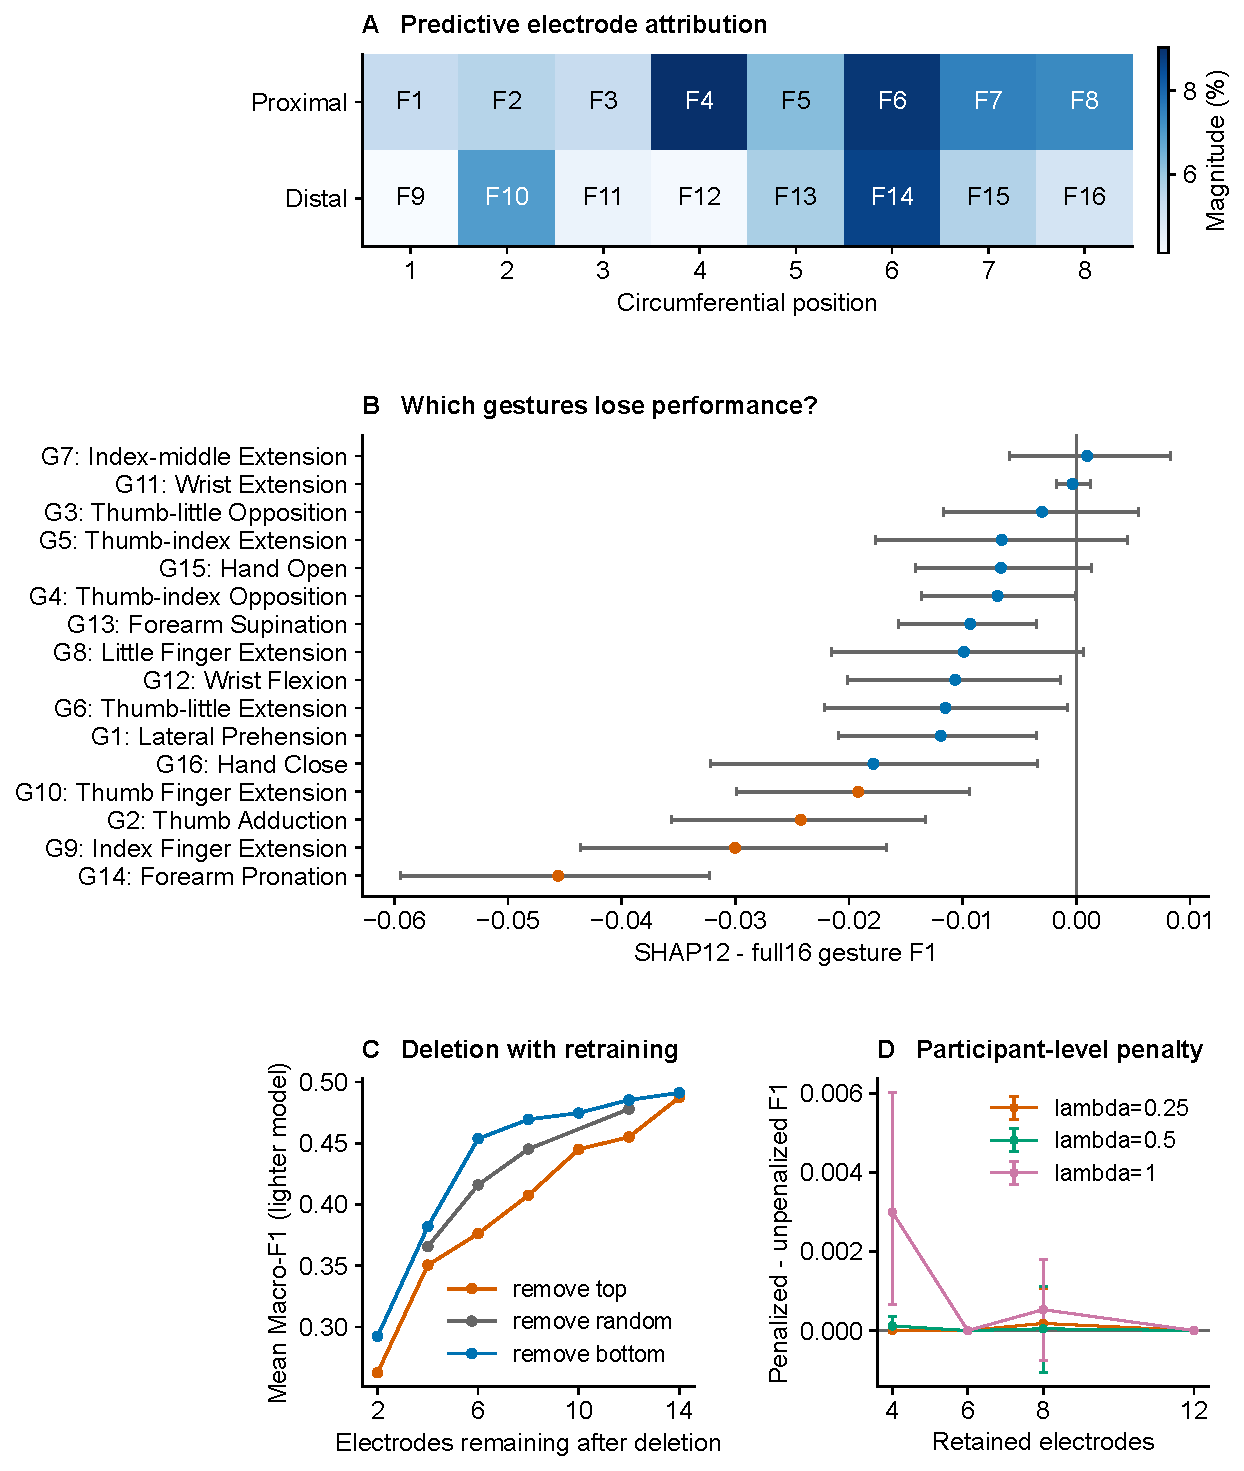
\includegraphics[width=\textwidth]{../figures/vector/fig5_task_and_attribution.pdf}
\caption{What the ranking represents and what reduction loses. (A) Mean fold-median normalized absolute attribution over outer folds on the documented topology; the scale is in percent and measures model relevance, not muscle activation. (B) Gesture-specific mean F1 changes with participant-bootstrap intervals; orange marks Holm-adjusted signed-rank $p<0.05$ across sixteen gestures. Names follow MotionSequence.txt, with paired-finger names shortened for display. (C) Deletion with retraining under the lighter model. (D) Participant-level aggregation, penalized minus unpenalized selection, with unadjusted 95\% paired mean-change intervals. Corrected signed-rank decisions are reported separately; a positive unadjusted mean interval is not a family-corrected penalty claim. Statistical families and differing model budgets are specified in Methods.}
\label{fig:task}\end{figure}

\subsection{Where does the electrode-count conclusion stop generalizing?}
The two split-derived fixed layouts gave different results. Odd-ID development/even-ID testing removed \FixedDropped, with change \FixedDiff\ (\FixedLCB\ to \FixedUCB), meeting the 0.02 criterion. The reverse removed \FixedSwapDropped, with change \FixedSwapDiff\ (\FixedSwapLCBSix\ to \FixedSwapUCB), whose lower bound missed the criterion. The reverse split met the percentile criterion in \RevFixedSwapSeedHits\ of \RevFixedSwapSeedN\ bootstrap seed reruns (\RevFixedSwapSeedPercent\%); this indicates numerical decision fragility, not a probability that NI is true. The original seed decision is retained. These are two layouts rather than one layout validated twice; the count had already been chosen using the full cohort. Neither is an independent prospective validation.

Rest-inclusive, window-length and fixed-count random-forest sensitivities compare reduced systems with their own full arrays (table~\ref{tab:sensitivity}; figure~\ref{fig:limits}(B)). Complete window and rest curves appear in the Supplementary. They reuse the primary ranking and test robustness of reduced-model evaluation; they do not show that newly estimated rankings would be invariant to those changes. The random-forest check has no estimated minimum count because only twelve and sixteen were tested.

DB5 provided a small, separate-data test. Its count-12 lower bound under the historical percentile criterion was \DBFiveDeltaKTwelveLCBSix, close to the 0.02 boundary, and no count met the historical Holm rule at that margin. The exploratory null-centred Holm analysis likewise supported no reduced count, even at the looser 0.03 margin. With only \DBFiveSubjects\ participants and different hardware/tasks, it offers an uncertain boundary assessment rather than confirmation of the GRABMyo count. Derived bipolar pairs likewise failed to support a reduction from eight to seven at the primary margin. This representation cannot validate an equivalent reduction in physical bipolar sensors.

Full-array cross-session comparisons did not isolate placement displacement or reduced-layout robustness. Their participant results are retained in the Supplementary. A future independently collected same-montage cohort would be needed to validate a locked common layout, electrode count and online performance.

\begin{table}[htbp]
\centering\small
\caption{Within-condition reduced minus full-array comparisons at the 0.02 margin. Null denotes the exploratory null-centred studentized bootstrap with Holm correction across tested counts. The RF experiment tests only 12 and 16 electrodes, so it estimates no minimum count.}\label{tab:sensitivity}
\begin{adjustbox}{max width=\textwidth}
\begin{tabular}{lllllll}\toprule
Condition & $n$ & $k$ & $\bar\Delta$ & 95\% CI & $k^*_{\rm CI}$ & $k^*_{\rm null}$\\\midrule
Primary 250 ms & 43 & 12 & -0.0133 & [-0.0160, -0.0106] & 12 & 12\\
Rest included & 43 & 12 & -0.0139 & [-0.0166, -0.0111] & 12 & 12\\
150 ms & 43 & 12 & -0.0119 & [-0.0145, -0.0093] & 12 & 12\\
500 ms & 43 & 12 & -0.0126 & [-0.0161, -0.0091] & 12 & 12\\
NinaPro DB5 & 10 & 12 & -0.0126 & [-0.0200, -0.0056] & 12 & none\\
Derived bipolar & 43 & 7 & -0.0158 & [-0.0203, -0.0113] & none & none\\
Random forest & 43 & 12 & -0.0078 & [-0.0104, -0.0052] & not estimated & not estimated\\
\bottomrule\end{tabular}
\end{adjustbox}
\end{table}

\begin{figure}[htbp]\centering
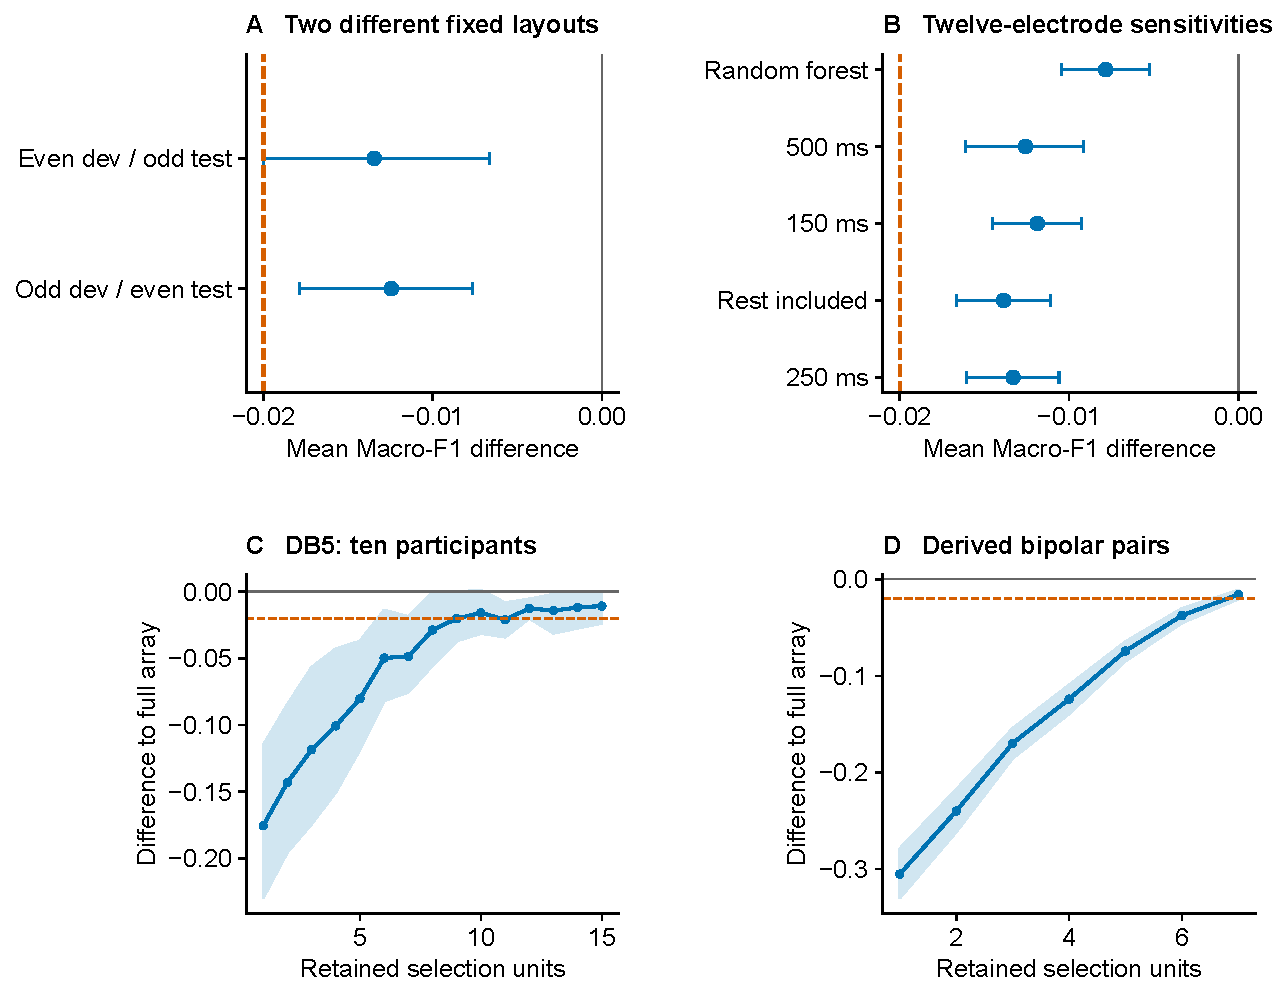
\includegraphics[width=\textwidth]{../figures/vector/fig6_generalization_limits.pdf}
\caption{Boundaries of transfer. (A) Mean changes and intervals for two distinct split-derived layouts, using 21 and 22 test participants and all development windows for fitting. (B) Twelve-electrode changes for task, window and classifier sensitivities, with each condition's own sixteen-electrode reference. (C) DB5 reduction versus its sixteen-channel reference ($n=10$). (D) Derived bipolar reduction versus its eight-pair reference ($n=43$). The dashed line is the 0.02 margin. Every interval resamples participants; scores are not pooled across hardware or representations.}
\label{fig:limits}\end{figure}
